\subsection{What are \ab{} calculations?}

\begin{frame}[allowframebreaks]{What are \ab{} calculations?}
    \begin{definitionblock}{\ab{} calculation}
        A method of calculating atomic and molecular structure directly from the first
        principles of quantum mechanics, without using quantities derived from experiment
        as parameters.
    \end{definitionblock}

    If still confused, have a look at \href{https://youtu.be/-RomkxjlIcQ}{the introduction video of \texttt{DFTK.jl}}.

    Some typical \ab{} calculations:
    \begin{itemize}
        \item Electronic structure calculation
        \item Structure optimization, prediction, and search
        \item \textit{Ab initio} molecular dynamics
        \item Phonons and vibrational spectra calculation
        \item Many-body Green's functions
    \end{itemize}

    \framebreak

    \begin{figure}[H]
        \centering
        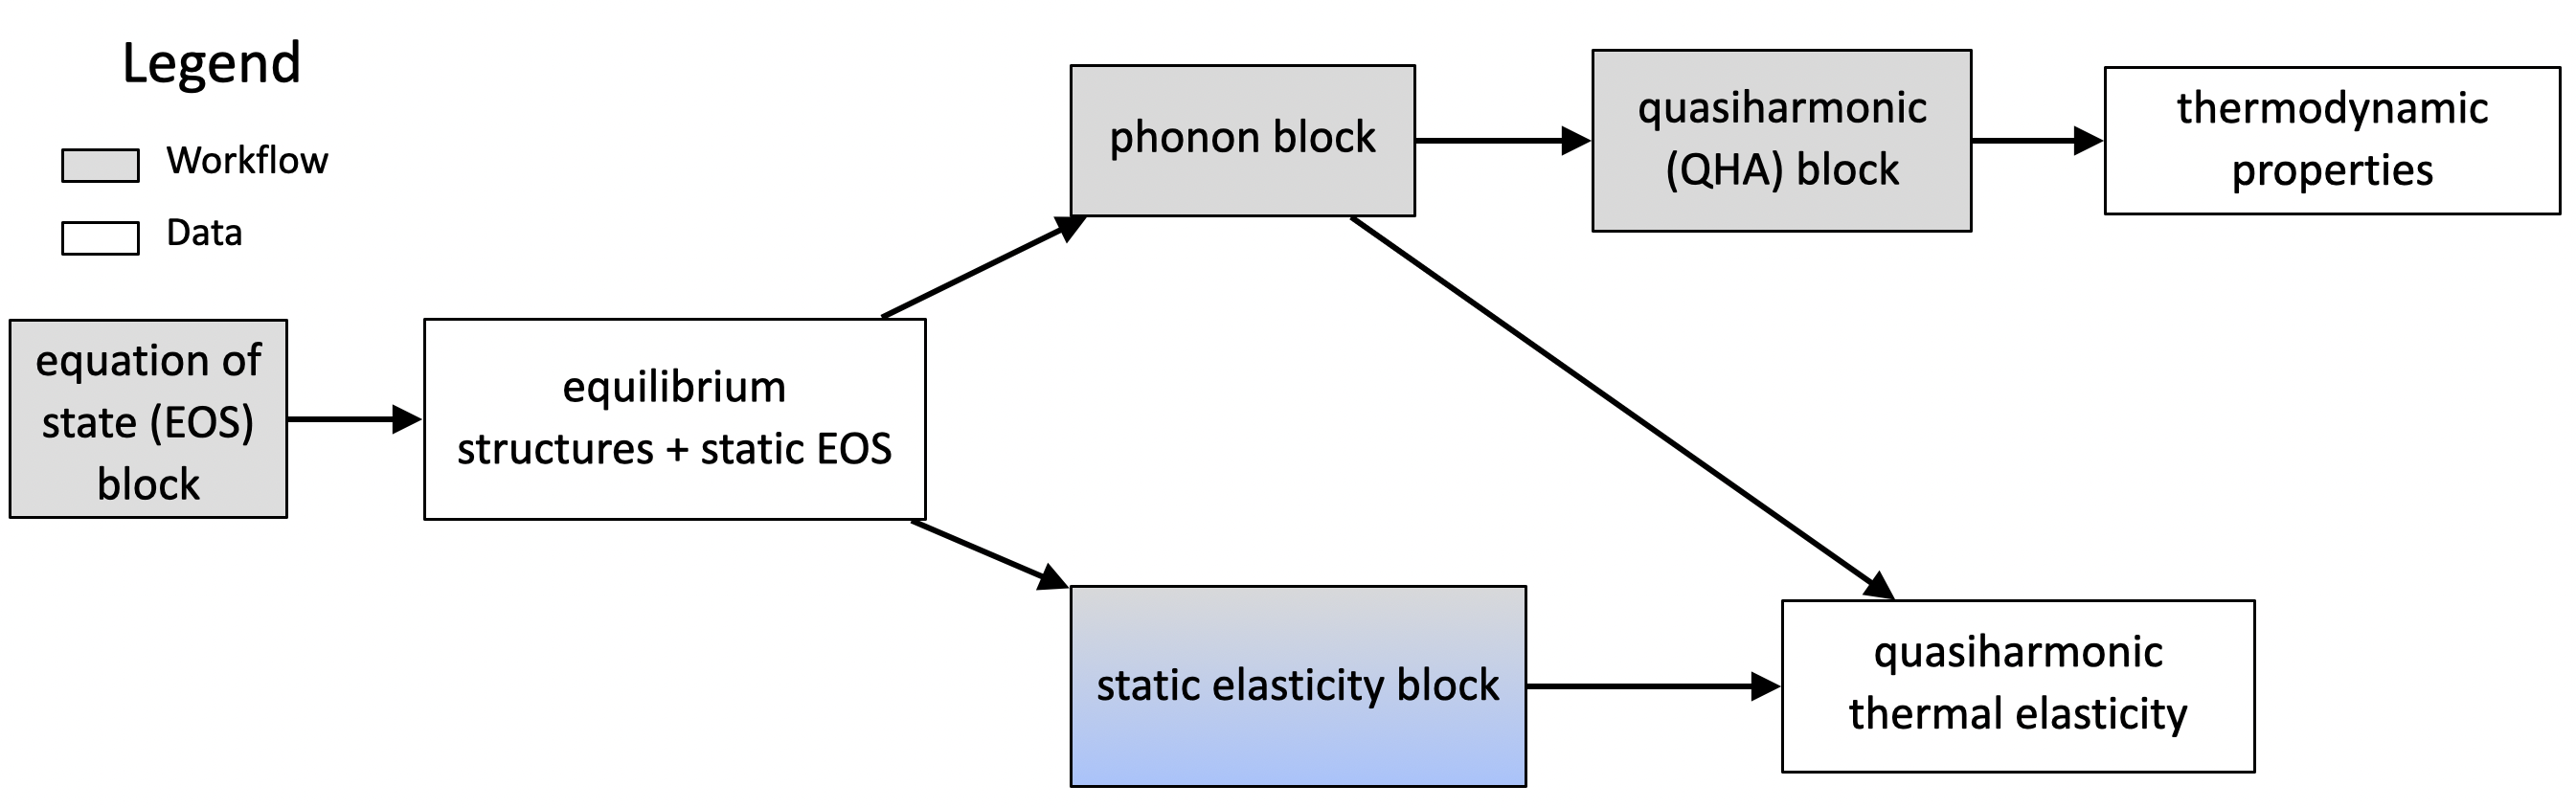
\includegraphics[height=0.4\textheight]{workflows}
        \caption{Typical \ab{} workflows used in our group}
        \label{eq:workflows}
    \end{figure}
\end{frame}

\begin{frame}{Various \ab{} software}
    To do \ab{} calculations, it is inevitable to interact with \ab{} software.
    There are a lot of them on the market, e.g., \qe{}, VASP, and ABINIT.
    They are often written in Fortran, and needed to be compiled to executable
    when using.

    So building a workflow for them requires us to create parsers for their input and output
    files, as well as functions to dynamically run these executables.

    \begin{figure}[b]
        \centering
        
\includegraphics[width=0.4\textwidth]{qe}
        \hfill
        
\includegraphics[width=0.2\textwidth]{vasp}
        \hfill
        
\includegraphics[width=0.3\textwidth]{abinit}
        \label{fig:abinitsoftware}
    \end{figure}
\end{frame}
